\chapter{Análisis y diseño}

\section{Análisis de requisitos}

Todo software se desarrolla para cubrir una necesidad, por lo que en este apartado vamos a describir los requisitos que se 
estiman necesarios para cubrir los objetivos propuestos.

\subsection{Descripción de los actores}

Los actores implicados serán dos: el \textbf{desarrollador} y el \textbf{usuario}.

\bigskip
El \textbf{desarrollador} será el encargado de solucionar los problemas de visualización de los datos en la plataforma, además de 
portar el desarrollo actual de la plataforma a un entorno de desarrollo continuo. También asumirá la administración de la 
plataforma ya que este tipo de rol está muy integrado con las labores de despliegue en el desarrollo continuo.

\bigskip
El \textbf{usuario} de la aplicación será cualquier persona que tenga interés por conocer datos internos de la Universidad de Granada 
fácilmente. El usuario no pertenece a ningún público objetivo concreto, por lo que no se tiene que considerar que tenga una
experiencia previa en navegador por sitios web.

\subsection{Requisitos Funcionales}

Los requisitos funcionales son las características que tiene que implementar el sistema para cubrir todas las necesidades de 
los distintos usuarios.

\bigskip
Al usuario lo único que le interesa es ver una página web estática con la información que desea 
consultar, para ello el desarrollador deberá hacer que sea posible que se generen siempre las tablas con los elementos de 
información. 

\bigskip
Por otra parte, el desarrollador quiere integrar el sistema en un desarrollo continuo, por lo que añadirá tests 
unitarios, test de cobertura, integración continua, despliegue automático y aprovisionamiento con tal fin.

\begin{itemize}
  \item \textbf{RF-1.} Administración de la plataforma:
    \begin{itemize}
    \item \textbf{RF-1.1.} Arrancar el portal mediante un script.
    \item \textbf{RF-1.2.} Detener el portal mediante un script.
    \end{itemize}
\end{itemize}

\begin{itemize}
  \item \textbf{RF-2.} Acceso a la información:
    \begin{itemize}
    \item \textbf{RF-2.1.} Consultar tablas con elementos de información.
    \end{itemize}
\end{itemize}

\begin{itemize}
  \item \textbf{RF-3.} Integración del desarrollo continuo:
  \begin{itemize}
    \item \textbf{RF-3.1.} Realizar tests unitarios.
    \item \textbf{RF-3.2.} Realizar test de cobertura.
    \item \textbf{RF-3.2.} Usar integración continua.
    \item \textbf{RF-3.3.} Usar despliegue automático.
    \item \textbf{RF-3.4.} Usar aprovisionamiento.
    \end{itemize}
\end{itemize}

\subsection{Requisitos no Funcionales}

Los requisitos no funcionales son las características propias del desarrollo, pero que no tienen que estar relacionadas con su 
funcionalidad.

\begin{itemize}
  \item \textbf{RN-1.} Toda la programación del portal se hará en Node.js y los módulos que se usen deben ser instalables a 
  través de su gestor de paquetes NPM.
  \item \textbf{RN-2.} El portal se iniciará y se detendrá mediante scripts lanzados con NPM.
  \item \textbf{RN-3.} Para iniciar la ejecución del portal es necesario que reciba el puerto de escucha del servidor y la 
  dirección de acceso.
  \item \textbf{RN-4.} Todos los módulos se ejecutarán desde scripts lanzamos con NPM.
  \item \textbf{RN-5.} Los tests unitarios se realizarán en base a comportamientos esperados y valores de estados
  recibidos como contestación a las peticiones que se realicen al portal.
  \item \textbf{RN-6.} Los tests unitarios tienen que recibir las páginas del portal para ejecutarse.
  \item \textbf{RN-7.} El test de cobertura tiene que tener una automatización integrable con los tests unitarios. 
  \item \textbf{RN-8.} La integración continua se ejecutará automáticamente con cada cambio que se haga en la programación
  del portal.
  \item \textbf{RN-9.} El despliegue automático se realizará mediante conexiones SSH.
  \item \textbf{RN-10.} Tanto para el despliegue automático como para el aprovisionamiento es necesario indicar el usuario que
  lo realiza y el destino en el que se realiza.
\end{itemize}

\subsection{Requisitos de Información}

Los requisitos de información se refieren a la información que es necesaria almacenar en el sistema. La única información 
relevante que se va a almacenar son los datos descriptivos y de enlace de cada uno de los elementos del portal OpenData UGR 
que se van a mostrar en UGR Transparente.

\begin{itemize}
  \item \textbf{RI-1.} Datos abiertos.
  \begin{itemize}
    \item Información sobre cada uno de los elementos que se van a mostrar en el portal de transparencia como datos abiertos.
    \item Contenido: nombre, categoría, conjunto de datos, enlace a OpenData UGR, enlace al recurso.
  \end{itemize}
\end{itemize}

\section{Modelos de casos de uso}

Aunque ya se ha indicado que la parte funcional ya se encuentra implementada de forma previa a este proyecto, se van a incluir
unos modelos de caso de uso simples para dar un visión más clara del funcionamiento general de la plataforma UGR Transparente.

\subsection{Descripción básica de actores}

\begin{itemize}
  \item \textbf{Ac-1.} Desarrollador
  \begin{itemize}
   \item Descripción: Encargado del desarrollo y administración de la plataforma.
   \item Características: Su trabajo está en el lado del servidor que genera la página, nunca trabaja desde el lado del cliente.
   \item Relaciones: Ninguna.
   \item Atributos: Ninguno.
   \item Comentarios: Es el encargado de que la información se muestre en el portal y de añadir funcionalidades a la plataforma.
  \end{itemize}
  
  \item \textbf{Ac-2.} Usuario
  \begin{itemize}
   \item Descripción: Persona que usa la plataforma que consulta datos.
   \item Características: Es el usuario común que accederá a la página.
   \item Relaciones: Ninguna.
   \item Atributos: Ninguno.
   \item Comentarios: El usuario no es necesario que tenga ningún conocimiento previo al uso de la plataforma, simplemente
   accederá y consultará los datos que sean de su interes.
  \end{itemize}
\end{itemize}

\subsection{Descripción casos de uso}

\begin{itemize}
  \item \textbf{CU-1.} Iniciar plataforma
  \begin{itemize}
    \item Actores: Desarrollador
    \item Tipo: Primario, Esencial
    \item Precondición: Ninguna
    \item Postcondición: El portal será accesible públicamente.
    \item Propósito: Arrancar el servidor del portal UGR Transparente.
    \item Resumen: Cuando se ejecuta el script de inicio de la aplicación, arranca el servidor y el portal será accesible desde
  internet.
 \end{itemize}
 
  \item \textbf{CU-2.} Detener plataforma
  \begin{itemize}
    \item Actores: Desarrollador
    \item Tipo: Primario, Esencial
    \item Precondición: La plataforma esté en ejecución.
    \item Postcondición: El portal deja de estar operativo.
    \item Propósito: Detener el servidor del portal UGR Transparente.
    \item Resumen: Cuando se ejecuta el script de detención de la aplicación, se detiene el servidor y el portal deja de estar
    accesible desde internet.
 \end{itemize}
 
 \newpage
 \item \textbf{CU-3.} Consultar datos
  \begin{itemize}
    \item Actores: Usuario
    \item Tipo: Primario, Esencial
    \item Precondición: Existan archivos con los datos abiertos.
    \item Postcondición:
    \item Propósito: El usuario consulta los datos mostrador en el portal UGR Transparente.
    \item Resumen: El usuario que accede al portal de transparencia, navega a través de las distintas categorías y selecciona
    aquella información que está interesado en conocer.
 \end{itemize}
 
 \item \textbf{CU-4.} Realizar tests unitarios
  \begin{itemize}
    \item Actores: Desarrollador
    \item Tipo: Primario, Esencial
    \item Precondición: Existan las páginas del portal de transparencia.
    \item Postcondición: 
    \item Propósito: Realizar tests unitarios para comprobar las funcionalidades de la aplicación.
    \item Resumen: Cada vez que se añadan nuevas páginas o funcionalidades al portal, se comprueba que funcionan correctamente.
 \end{itemize}
 
 \item \textbf{CU-5.} Realizar tests de cobertura
  \begin{itemize}
    \item Actores: Desarrollador
    \item Tipo: Primario, Esencial
    \item Precondición: Existan tests unitarios
    \item Postcondición: 
    \item Propósito: Realizar test de cobertura para comprobar calidad de los tests unitarios.
    \item Resumen: Para comprobar si los tests unitarios cumplen correctamente con su función se analiza el porcentaje del
    código que está cubierto por los mismos.
 \end{itemize}
 
 \newpage
 \item \textbf{CU-6.} Usar integración continua
  \begin{itemize}
    \item Actores: Desarrollador
    \item Tipo: Primario, Esencial
    \item Precondición: Existan test unitarios.
    \item Postcondición: Se genera un informe con el resultado de los tests unitarios.
    \item Propósito: Comprobar si los cambios en la aplicación provocan errores.
    \item Resumen: Cuando se efectúan cambios en la aplicación automáticamente se ejecutan los tests unitarios para comprobar si
    los cambios introcudidos provocan conflictos en la plataforma.
 \end{itemize}
 
 \item \textbf{CU-.7 } Usar despliegue continuo
  \begin{itemize}
    \item Actores: Desarrollador
    \item Tipo: Primario, Esencial
    \item Precondición: 
    \item Postcondición: Los cambios introducidos son aplicados en la plataforma.
    \item Propósito: Aplicar automáticamente los cambios realizados a la aplicación. 
    \item Resumen: Para no tener que acceder manualmente al servidor de la plataforma y tener que desplegar los cambios 
    introducidos, desde el entorno de desarrollo desplegamos automáticamente los cambios en el servidor.
 \end{itemize}
 
 \item \textbf{CU-.8 } Usar aprovisionamiento
  \begin{itemize}
    \item Actores: Desarrollador
    \item Tipo: Primario, Esencial
    \item Precondición: 
    \item Postcondición: El portal queda instalado en la infraestructura seleccionada.
    \item Propósito: Instalar automáticamente el portal en una infraestructura dada.
    \item Resumen: Se instalarán automáticamente todos los elementos necesarios para poner en funcionamiento el portal en 
    cualquier infraestructura que se indique.
 \end{itemize}


\subsection{Diagramas de casos de uso}

Para tener una visión más facil de como se comportan las funcionalidades que vamos a añadir al portal en el diagrama de casos 
de uso podemos ver como se relacionan los diferentes casos de uso entre si y con los distintos actores que intervienen.

\begin{figure}[!h]
  \begin{center}
  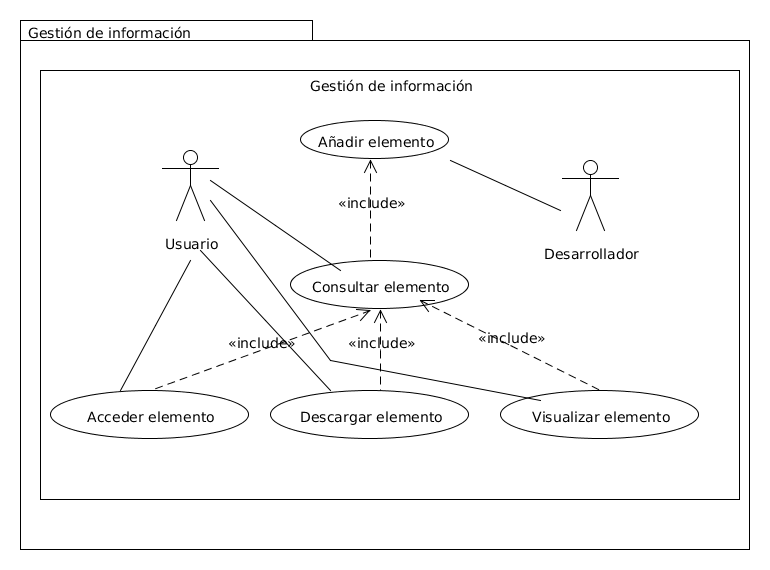
\includegraphics[width=1\textwidth]{imagenes/diagrama_casos_uso.png}
  \caption[Casos de uso]{Diagrama de casos de uso}
  \label{fig:casosUso}
  \end{center}
\end{figure}

